\section{Light Collection}
\label{sec:studies_light-col}

For the \AC{} detector concept detailed in Section~\ref{sec:ac_argoncube}, a slim and efficient light readout is needed.
\glspl{pmt} are not suitable because they occupy a lot of space and thus would require mounting on top of a module which in turn would reduce their efficiency.
That is why the photon detectors of choice for such a detector are \glspl{sipm}.
The following describes the light readout used in the \AC{} pixel demonstrator described in Section~\ref{sec:ac_viper}.
After that the \AC{} Light readout, \AL{}, is introduced.


\subsection{Cryogenic \glsentryshort{sipm} Light Readout}
\label{sec:studies_light-col_viper}

In 2016, the University of Bern developed a novel cosmic ray tagger system for \lartpc{}s which was subsequently installed in \uboone{}~\cite{uboone} and will be installed in the \sbnd{} experiment~\cite{sbnd} in the near future.
The tagger consists of panels made from polystyrene based scintillating bars.
On both long edges of the strips, the light is coupled into a \emph{Kuraray Y11(200)M}\footnote{\url{http://kuraraypsf.jp}} wavelength-shifting (WLS) fibre of \SI{1}{\milli\metre} diameter.
One end of the fibre is coated with an aluminium mirror to increase collection efficiency.
The other end is attached to a \emph{Hamamatsu S12825-050P}\footnote{\url{http://www.hamamatsu.com}} \gls{sipm}.
A bespoke Front-End Board (FEB) reads out the \gls{sipm} signal and provides power.
It was developed at LHEP at the University of Bern alongside the scintillator panels\cite{crt_feb}.

For the first pixel prototype described in Section~\ref{sec:ac_viper}, the CRT system was adapted to serve as the light trigger system.
Except for operating everything up to the \glspl{sipm} in \lar{}, the polystyrene scintillating bars were replaced by acrylic rings.
The latter are placed in between the aluminium field shaping rings of the \gls{tpc}.
To allow for proper convection of the \lar{}, only every other gap is completely filled by an acrylic ring.
Perpendicularly to the rings(i.e.\ in drift direction), four WLS fibres collect the light from the rings and guide it to the readout plane on the anode side where it is fed to the \glspl{sipm}.
Residing on the cryostat top-flange at room temperature, the front-end board is connected to the \glspl{sipm} via Teflon insulated coaxial cables.

The peak of scintillation light emission in \lar{} lies at \SI{128}{\nano\metre}\todo{sauce} while the sensitivity wavelength peak of the \gls{sipm} is at \SI{450}{\nano\metre}.
Therefore, the scintillation light needs to be shifted before it can be detected by the \glspl{sipm}.
This happens in two stages.
For the first shift, tetraphenyl butadiene (TPB) is applied to the inside of the acrylic rings.
Their outside is not coated to reduce the collected amount of scintillation light that originates outside the \gls{tpc} while their inside is machined to optimise light collection.
TPB absorbs the \SI{128}{\nano\metre} scintillation light an re-emits with a peak at \SI{440}{\nano\metre}~\cite{tpb} which is then propagated through the acrylic and coupled into the WLS fibre.
The latter has an absorption peak at \SI{430}{\nano\metre} and an emission peak at \SI{476}{\nano\metre}.\todo{sauce}

In the front-end board, two coincidences of two out of four \glspl{sipm} are formed and combined by means of a logic \emph{OR} operation.
The trigger pattern is thus
\begin{IEEEeqnarray}{rCl}
	T & = & \qty(S_1 \land S_2) \lor \qty(S_3 \land S_4)
\end{IEEEeqnarray}
for \glspl{sipm} $S_1$ through $S_4$.
The reason for this is that the same trigger logic is used for the CRT panels to have a coincidence between two fibres of one scintillation bar.
In order to improve trigger purity, it was tried to change the firmware to trigger on the coincidence of all four fibres in the \gls{tpc}.
Due to a firmware bug however this could not be achieved.

As will be explained in Section~\ref{sec:ac_viper}, the light readout scheme described above was successfully used to trigger and record several thousand cosmic muon interactions with the \AC{} pixel demonstrator.
However, when compared to a measurement triggered on the charge readout directly, it became apparent that the efficiency of this light readout is very poor.
Due to limitations in the experimental setup, no quantitative measurement of the trigger efficiency was performed.
Triggering on the charge readout was only possible using an oscilloscope because the used DAQ system was not capable of self-triggering.
Therefore the channel number was limited to four which would have enabled charge readout triggering only on a subset of the readout area.
An external reference trigger source, such as a muon telescope was not available during the measurements.
Furthermore, after warming up the experiment, it was discovered that all four fibres were damaged because the acrylic rings fell out of their mounting brackets and squeezed or even broke the corresponding fibre.

Another drawback of the design is the optical coupling between the acrylic rings and the \lar{}.
Because the refractive indices are very close, a lot of light escapes from the rings and is lost.
Many other low-volume light readout systems based on light guides developed for \lar{}~\cite{lar_lro1, lar_lro2, lar_lro3, lar_lro4, lar_lro5, lar_lro6, lar_lro7} suffer from the same problem.
As a solution, a dedicated light readout system for the \AC{}, \AL{}, was developed at the University of Bern.


\subsection{\glsentryshort{arclight}}
\label{sec:studies_light-col_al}
\glsreset{arclight}

The \AL{} aims to minimise the occupied volume by maximising the area coverage of \glspl{sipm}.
This is achieved by coupling them to a passive light collector.
As mentioned above, principles based on full reflection on a polymer-\lar{} interface are not suitable.
Instead, \AL{} is based on the light trapping principle of the ARAPUCA sensor~\cite{arapuca}.
The latter works by trapping the photons inside a cavity made of walls covered by a highly reflective materials.
One of the walls is formed from a dichroic film, a material transparent to certain wavelengths while highly reflective to others.
On the outside, this film is covered by TPB with the film transparent to the emitted blue light.
The inside of the film is covered by a second WLS, shifting the light to green which is reflected by the dichroic film and therefore trapped inside the cavity.
One or more \glspl{sipm} are mounted inside the cavity to collect the trapped photons.
In contrast, \AL{} replaces the void of ARAPUCA by a solid transparent polymer sheet, doped with a WLS dye.
This makes it substantially more robust, compact and stable, especially when scaled up to larger areas.

\begin{figure}[htb]
	\centering
	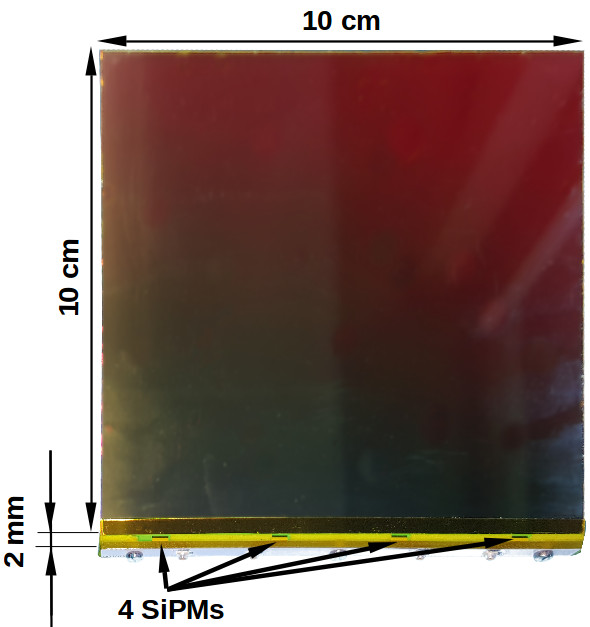
\includegraphics[width=.5\textwidth]{arclight/prototype}
	\caption{\SI{10 x 10}{\centi\metre} \AL{} prototype.
		Four \glspl{sipm} can be seen at the lower side, soldered to a narrow \gls{pcb} providing coaxial connectors for signal readout.
		The rest of the sensor area is dielectric.}
	\label{fig:arclight_prototype}
\end{figure}

A \SI{10 x 10}{\centi\metre} \AL{} prototype is shown in Figure~\ref{fig:arclight_prototype}.
The ratio of sensitive area to total area is \SI{98}{\percent} with the remaining \SI{2}{\percent} occupied by a \gls{pcb} carrying four \emph{Hamamatsu S13360-3050VE}\footnote{\url{http://www.hamamatsu.com}} \glspl{sipm} with a sensitive area of \SI{3 x 3}{\milli\metre} each.
The inside of \AL{} is made of a \SI{4}{\milli\metre} thick \emph{Eljen Technology EJ-280}\footnote{\url{http://www.eljentechnology.com}} WLS plate.
Its sides are laminated with reflective films.
The back face and the edges are covered with a \emph{3M VM2000}\footnote{\url{https://www.3m.com}\label{foot:3M}} dielectric specular reflector foil having $\approx \SI{98}{\percent}$ reflectance in the visible light range.
A \emph{3M DF-PA Chill}\textsuperscript{\ref{foot:3M}} dichroic mirror covers the front face.
It is transparent in the blue and has a high reflectance in the green spectral range.
Both films are held in place by thin layers of transparent adhesive.
To shift the vacuum UV (VUV) scintillation light produced in \lar{} to the blue transparent range of the dichroic mirror, its outer surface is coated with TPB.
A cross-section of the structure of \AL{} is depicted in Figure~\ref{fig:arclight_structure}.

\begin{figure}[htb]
	\centering
	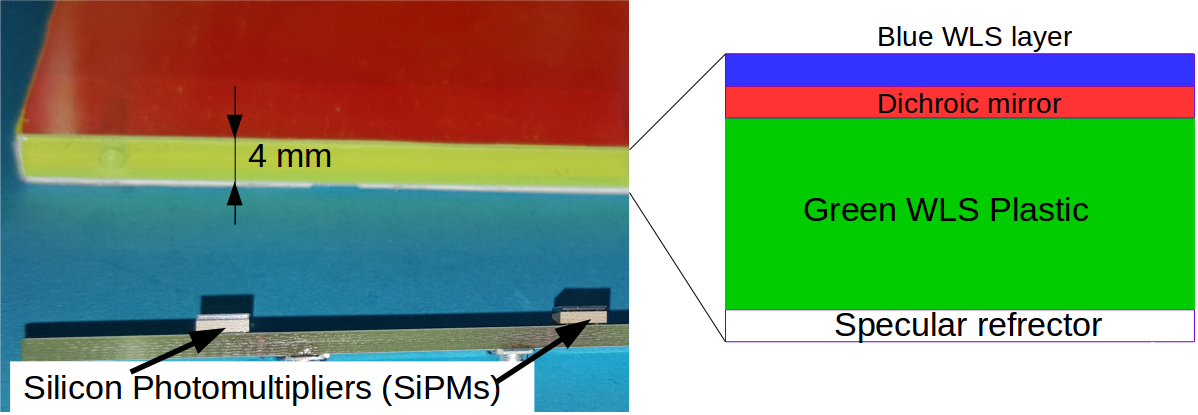
\includegraphics[width=\textwidth]{arclight/structure}
	\caption{\AL{} light collector cross-section near a corner.
		The structure is mechanically supported by a \SI{4}{\milli\metre} thick WLS plastic.
		Its front is covered with a dichroic mirror film while the edges and the back face are covered with a dielectric specular reflector foil.
		The outer surface of the dichroic mirror is coated with TPB to shift the \lar{} VUV scintillation light to the blue range where the dichroic film is transparent.
		At the bottom of the left picture, two of the four \glspl{sipm} mounted to the carrier \gls{pcb} are visible.}
	\label{fig:arclight_structure}
\end{figure}

The Photon Detection Efficiency (PDE) was measured at room temperature using an \ce{^241 Am} source, previously calibrated with a \gls{pmt}.
It was determined to be \SIrange{0.8}{2.2}{\percent}.
Figure~\ref{fig:arclight_pde} shows PDE as a function of the position inside the light collector, overlaid onto a picture of the prototype for reference.
The increase in PDE near the \glspl{sipm} is likely caused by photons hitting the \glspl{sipm} directly with no prior reflection off the dichoic mirror.
Due to the angular dependence of the reflectance of the dichroic mirror, about \SI{30}{\percent} of the light is lost during the first reflection on the dichroic mirror.
Once reflected, a photon is trapped inside the \AL{} because of the specular nature of the reflection on all surfaces.
In addition, the average PDE was calculated from theory to be \SI{0.7 +- 0.4}{\percent} in agreement with the measurements.
More details on the calculations and the calibration of the measurement can be found in~\cite{arclight}.

\begin{figure}[htb]
	\centering
	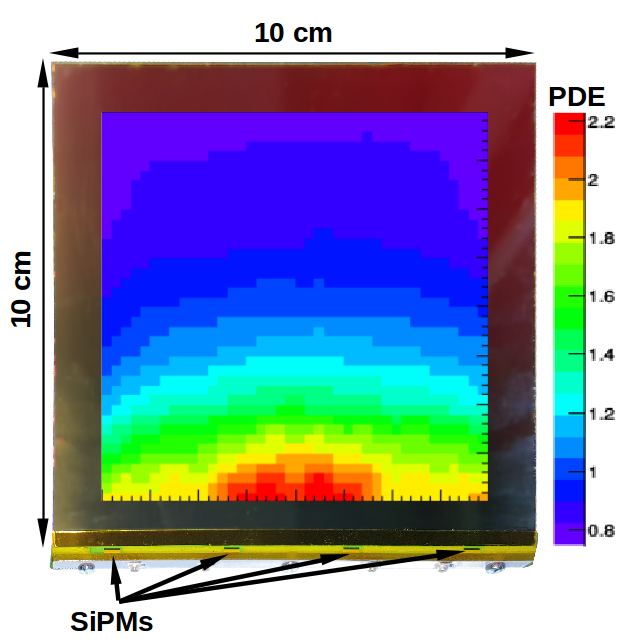
\includegraphics[width=\textwidth]{arclight/PDE}
	\caption{Measured photon detection efficiency (PDE) for the \SI{10 x 10}{\centi\metre} \AL{} prototype (in the background), at room temperature.
		The PDE is given in \si{\percent}.
		Near the \glspl{sipm} at the bottom, the PDE is increased due to an increased fraction of direct photons, avoiding the initial loss at the first reflection from the dichroic mirror.}
	\label{fig:arclight_pde}
\end{figure}

The measurements described above were performed at room temperature.
A \SI{43 x 15}{\centi\metre} \AL{} module was successfully operated at \lar{} temperatures in the \pixlar{} test beam demonstrator at FNAL described in Section~\ref{sec:ac_pixlar}.
Figure~\ref{fig:arclight_pixlar} shows the time evolution of the average photo-electron yield per event in beam (red) and cosmic ray (blue) mode.
It can be seen that the yield is approximately constant over several weeks.
The jumps in the beam curve can be explained by the switching between different beam configurations (e.g.\ momentum and intensity).


\begin{figure}[htb]
	\centering
	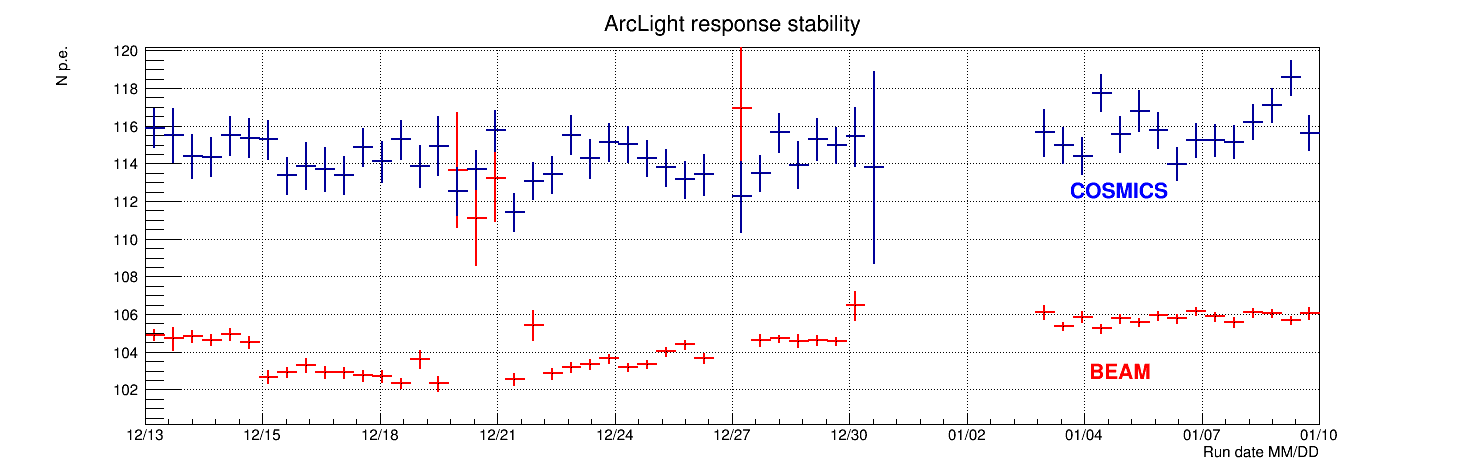
\includegraphics[width=\textwidth]{arclight/stability_cosm_beam}
	\caption{Average observed number of photo-electrons (N p.e.) per event by the \AL{} module in the \pixlar{} test beam demonstrator at FNAL over several weeks.
		In addition to the beam response in red, the response to cosmic rays is shown in blue.}
	\label{fig:arclight_pixlar}
\end{figure}